\documentclass[xcolor={x11names,svgnames,psnames}]{beamer}

\usepackage[T1]{fontenc}
\usepackage{cellspace}

\usepackage{amsmath}
\usepackage{amsfonts}
\usepackage{tikz}
\usepackage{xspace}
\usepackage[normalem]{ulem}
\usepackage{minted}

\usepackage{marvosym}
\usepackage{pifont}

\newcommand{\bigO}[1]{\ensuremath{\mathcal{O}\left( #1 \right)} }
\newcommand{\triste}{\includegraphics[width=0.5cm,trim=0 17mm 0 0]{triste}}

\newcommand{\red}{\alert}
\newcommand{\green}{\color{LimeGreen}}
\newcommand{\blue}{\color{cyan}}

% FORTIN
\newcommand{\mynote}[1]{\note<1>[item]{#1}}
\newcommand{\euro}{\EUR\xspace}

\usetikzlibrary{patterns}
\usetikzlibrary{snakes}
 \usetikzlibrary{arrows}
\usetikzlibrary{backgrounds}
\usetikzlibrary{shapes}
\usetikzlibrary{shadows}
\usetikzlibrary{calc}
\usetikzlibrary{decorations}
\usetikzlibrary{decorations.pathmorphing}
\usetikzlibrary{decorations.shapes}
\usetikzlibrary{decorations.markings}
\usetikzlibrary{positioning}

\definecolor{amethyst}{rgb}{0.6, 0.4, 0.8}
\definecolor{cyan}{rgb}{0,0.6796875,1}

\usecolortheme{rose}
\setbeamertemplate{footline}{}
\setbeamertemplate{navigation symbols}{}

\usepackage{fontspec}

\setsansfont{PalatinoSansLTPro}[
   Path = /home/charles/charles_work/fonts/PalatinoSans/, 
   Extension      = .otf,
   UprightFont    = *-Regular,
   BoldFont= *-Bold ,
   ItalicFont = *-Italic,
   BoldItalicFont = *-BoldIta
]

%\author[C.~Bouillaguet]{Charles Bouillaguet \newline
%  {\small (\texttt{charles.bouillaguet@lip6.fr})}}

\title{Lecture \# 1 : Introduction}
%\date{2020-01-27}

\begin{document}


%%%%%%%%%%%%%%%%%%%%%%%%%%%%%%%%%%%%%%%%%%%%%%%%%%%%%%%%%%%%%%%%%%%%%

\section{Introduction blabla}

\begin{frame}[label=title]
  \titlepage
\end{frame}
 
 
%%%%%%%%%%%%%%%%%%%%%%%%%%%%%%%%%%%%%%%%%%%%%%%%%%%%%%%%%%%%%%%%%%%%%

\begin{frame}
\frametitle{What is HPC ?}


\begin{alertblock}{\emph{High-Performance Computing} (HPC)}
  Mixture of
  \begin{enumerate}
  \item Specialized (parallel) hardware 
  \item Adapted (parallel) algorithms 
  \item \textit{Ad hoc} (parallel) programming techniques
  \end{enumerate}
\end{alertblock}

\medskip

+ Specially trained programmers !

\end{frame}


 

%%%%%%%%%%%%%%%%%%%%%%%%%%%%%%%%%%%%%%%%%%%%%%%%%%%%%%%%%%%%%%%%%%%%%
\begin{frame}
  \frametitle{Course Topics}
  
  \begin{enumerate}%[circle]
  \item Introduction
  \item Distributed programming using MPI
  \item Multi-thread programming with OpenMP
  \item Vectorization
  \item Understanding the hardware and exploiting its full capacity 
  \item Recurring algorithmic themes/problems
  \end{enumerate}

  \bigskip
  
  \alert{Next year: GPUs/accelerators} 
\end{frame}







%%%%%%%%%%%%%%%%%%%%%%%%%%%%%%%%%%%%%%%%%%%%%%%%%%%%%%%%%%%%%%%%%%%%%

\begin{frame}
\frametitle{Fundamental Role of Numerical Simulations}

\begin{block}{Traditional scientific method}
  \begin{enumerate}
  \item Formulation of a theory based on observations
  \item Design of experiments to (in)validate the theory
  \item Compare experimental results with observations
  \end{enumerate}
\end{block}

Iterate the process until convergence.

\begin{alertblock}{But experimenting can be too...}
  \begin{itemize}
  \item Difficult (\emph{Wind Tunnel} containing an Airbus A380?)
  \item Expensive (\emph{crash test}, ...)
  \item Slow (climate evolution, galaxy dynamics, ...)
  \item Dangerous (clinical trials, \Biohazard, \Radioactivity, \Laserbeam, ...)
  \end{itemize}
\end{alertblock}
\end{frame}

%%%%%%%%%%%%%%%%%%%%%%%%%%%%%%%%%%%%%%%%%%%%%%%%%%%%%%%%%%%%%%%%%%%%%%

\begin{frame}
  \frametitle{Numerical Simulations}

  \begin{exampleblock}{Using computers to simulate and analyze a physical phenomenon}
  
  \begin{columns}[t]
    \column{0.5\textwidth} 
    \begin{itemize}
    \item Starting from physical laws

      \medskip

    \item Using numerical methods

      \medskip
      
    \item with ever more powerful computers
    \end{itemize}
    
    \column{0.5\textwidth}
    \begin{center}
      \begin{figure}[ht]
        \centering
        \includegraphics[width=0.9\textwidth]{Science-SimuNum.pdf}
      \end{figure}
      {\tiny (after
        % {\it Parallel Programming in C 
        % with MPI and OpenMP}, 
        M.J. Quinn)} 
    \end{center}
  \end{columns}
\end{exampleblock}

\begin{itemize}
\item[$\leadsto$] 3rd pillar of science?
\end{itemize}  
\end{frame}


% %%%%%%%%%%%%%%%%%%%%%%%%%%%%%%%%%%%%%%%%%%%%%%%%%%%%%%%%%%%%%%%%%%%%%
% \begin{frame}
% \frametitle{Les grands domaines d'application du HPC}


% \begin{block}{``Grands challenges'' scientifiques}
%   \begin{itemize}
%   \item Chimie, biologie : dynamique moléculaire 
%   \item Bio-informatique : séquençage du génome
%   \item Astrophysique : dynamique des  galaxies, de l'Univers  
%   \item Climatologie : échanges océan $\leftrightarrow$ atmosphère
%   \item Méca. des fluides : écoulements turbulents, combustion
%   \item ...
%   \end{itemize}
% \end{block}

% Et aussi : 
% \begin{itemize}
% \item Géophysique : propagation d'ondes sismiques
% \item Industrie automobile : simulation d'accidents 
% \item \og \textit{Deep Learning}\fg
% \item ... 
% \end{itemize}
% \end{frame}

%%%%%%%%%%%%%%%%%%%%%%%%%%%%%%%%%%%%%%%%%%%%%%%%%%%%%%%%%%%%%%%%%%%%%

\begin{frame}
\frametitle{Illustration of the Problem}

\begin{center}
\includegraphics[width=5cm]{earth-core.jpg}
\end{center}

\begin{itemize}
\item surface = 510 millions km${^2}$, volume $\approx 10^{12}$ km${}^3$
  \medskip
\item One \texttt{double} per km${}^3$ $\leadsto$ 8 TB of memory

\item One \texttt{double} per m${}^2$ $\leadsto$ 4 PB of memory
\end{itemize}

\end{frame}

%%%%%%%%%%%%%%%%%%%%%%%%%%%%%%%%%%%%%%%%%%%%%%%%%%%%%%%%%%%%%%%%%%%%%

\begin{frame}
\frametitle{Illustration of the Problem (continued)}

\begin{center}
\includegraphics[width=5cm]{cell.jpg}
\end{center}

\begin{itemize}
\item Human cell. About $10^{14}$ atoms.
\item 3 $\times$ \texttt{double} $(x, y, z)$ per atom $\leadsto$ 2.4 PB of memory
\end{itemize}

\medskip

\begin{alertblock}{Not to mention...}
  \begin{itemize}
  \item $10^{11}$--$10^{12}$ stars in out galaxy
  \item $10^{11}$--$10^{12}$ galaxies...
  \end{itemize}
\end{alertblock}

\end{frame}


%%%%%%%%%%%%%%%%%%%%%%%%%%%%%%%%%%%%%%%%%%%%%%%%%%%%%%%%%%%%%%%%%%%%%%

\begin{frame}
  \frametitle{Realization \triste}

  \begin{itemize}
  \item You know \textbf{a little} how does a computer work
    \begin{itemize}
    \item But \red{not completely}
    \item Especially the big ones
    \end{itemize}

    \medskip
    
  \item You have not been trained to :
    \begin{itemize}
    \item \red{Care} about the \textbf{performance} of your code
    \item Write \textbf{efficient} programs
    \end{itemize}
    
    \pause
    \bigskip

    \item \Huge \textbf{Time for a change}
    \end{itemize}

\end{frame}

%%%%%%%%%%%%%%%%%%%%%%%%%%%%%%%%%%%%%%%%%%%%%%%%%%%%%%%%%%%%%%%%%%%%%% 

\begin{frame}
  \frametitle{Computing Power}

  \begin{block}{performance measurement}
  Unit : FLOP (\textit{Floating Point OPeration}), FLOP/s (or FLOPS)

  \begin{itemize}
  \item Giga ($10^9 \approx 2^{30}$)
  \item Tera ($10^{12} \approx 2^{40}$)
  \item Peta ($10^{15} \approx 2^{50}$)
  \item Exa  ($10^{18} \approx 2^{60}$) \dots 
  \end{itemize}
\end{block}

\bigskip

\begin{itemize}
\item Machines for large computations = \textbf{\red{parallel} computers}

  \medskip

  \item Parallelism is an \textbf{inexorable trend}
  \end{itemize}
\end{frame}


%%%%%%%%%%%%%%%%%%%%%%%%%%%%%%%%%%%%%%%%%%%%%%%%%%%%%%%%%%%%%%%%%%%%%%
\section{HPC Hardware}


\begin{frame}
  \frametitle{1990's PC}
  \framesubtitle{The only one your really know how to program}
  
  \centering
  \includegraphics[height=0.5\textheight]{old_pc}
  \hfill
  \includegraphics[width=6cm]{2cv}

  \bigskip

  1 core, 25Mhz, 16KB cache, 4MB RAM
\end{frame}

%%%%%%%%%%%%%%%%%%%%%%%%%%%%%%%%%%%%%%%%%%%%%%%%%%%%%%

\begin{frame}
  \frametitle{Contemporary Laptop}
  \framesubtitle{What you own, fortunately}
  
  \centering
  \includegraphics[width=5cm]{laptop}%
  %\hfill%
  \includegraphics[width=6cm]{r5maxi}

    \bigskip

  4 cores, 4Ghz, 8MB cache, 16GB RAM (2 channels)
\end{frame}


\begin{frame}
  \frametitle{Gamer's PC}
  \framesubtitle{For smart-asses who think IA will replace actual science}
  
  \centering
  \includegraphics[width=5cm]{gamer}%
  \hfill%
  \includegraphics[width=5.5cm]{tuning}

    \bigskip

    10--16 cores, 4Ghz, 16MB cache, 32Go RAM (2 channels)
\end{frame}


\begin{frame}
  \frametitle{Compute Node}
  \framesubtitle{Now we're talking}
  
  \centering
  \includegraphics[width=5cm]{dell1}
  \includegraphics[width=5cm]{dell2}


  \includegraphics[width=8cm]{gt40}

  \bigskip

  2 CPUs, 32--128 cores, 2.5Ghz, 256Go RAM ($2\times$ 6--8 channels)
\end{frame}


\begin{frame}
  \frametitle{Supercomputer}
  \framesubtitle{Rare and Expensive}
  
  \centering
  \includegraphics[width=7cm]{bgp}
  \hfill
  \includegraphics[width=7cm]{f1}

  \bigskip
  
  1000--10000000 cores. Cost between $10^{6}$ and $10^{9}$ euros
\end{frame}

%%%%%%%%%%%%%%%%%%%%%%%%%%%%%%%

\begin{frame}
  \frametitle{Description of an HPC machine: \texttt{Turing}}
  \framesubtitle{IBM BlueGene/Q (2012--2019) @ IDRIS (CNRS)}
  
  \begin{center}
    \includegraphics[height=6.5cm]{turing}
  \end{center}
\end{frame}

%%%%%%%%%%%%%%%%%%%%%%%%%

\begin{frame}
  \frametitle{Description of an HPC machine: \texttt{Turing}}
  \framesubtitle{IBM BlueGene/Q (2012--2019) @ IDRIS (CNRS)}

  6 racks, 98~304 cores (``small'') $\leadsto$ \texttt{Sequoia} (USA) has 1~572~864
  
  \begin{center}
    \includegraphics[width=\textwidth]{bgq}
  \end{center}
\end{frame}

%%%%%%%%%%%%%%%%%%%%%%%%%%%%%%

\begin{frame}
  \frametitle{Description of an HPC machine: \texttt{Turing}}
  \framesubtitle{IBM BlueGene/Q (2012--2019) @ IDRIS (CNRS)}
  
  \begin{columns}
    \begin{column}{0.33\textwidth}
      1 rack =
      \begin{itemize}
      \item 16 \textit{node cards}
      \item + power feeds
      \item + \textit{water cooling}
      \item + I/O nodes
      \end{itemize}

      \bigskip
      
      Total =
      \begin{itemize}
      \item 1024 nodes
      \item 16 384 cores
      \item 16 To de RAM
      \end{itemize}
      
    \end{column}
      
    \begin{column}{0.66\textwidth}
      \includegraphics[height=7.5cm]{bgqMidplane}
    \end{column}
  \end{columns}
\end{frame}

%%%%%%%%%%%%%%%%%%%%%%%%%%%%%%%%

\begin{frame}
    \frametitle{Description of an HPC machine: \texttt{Turing}}
  \framesubtitle{IBM BlueGene/Q (2012--2019) @ IDRIS (CNRS)}
  
  1 \textit{node card} = 32 \textit{compute cards}
  
  \begin{center}
    \includegraphics[height=6.5cm]{bgqNodeCard}
  \end{center}
\end{frame}


\begin{frame}
    \frametitle{Description of an HPC machine: \texttt{Turing}}
  \framesubtitle{IBM BlueGene/Q (2012--2019) @ IDRIS (CNRS)}
  
  1 \textit{compute card} =
  \begin{itemize}
  \item 1 PowerPC A2 CPU (16 cores @ 1.6Ghz, 32MB Cache)
  \item 16Go of ECC RAM (36 $\times$ 512MB chip)
  \end{itemize}

  \begin{center}
    \includegraphics[width=\textwidth]{bgqComputeCard}
  \end{center}
\end{frame}

% \begin{frame}
%   \frametitle{Description of an HPC machine: \texttt{Turing}}
%   \framesubtitle{IBM BlueGene/Q (2012--2019) @ IDRIS (CNRS)}

%     \includegraphics[width=\textwidth]{lstopo_bgq}
% \end{frame}

%%%%%%%%%%%%%%%%%%%%%%%%%%%%%%%%%%%%%%%%%%%%%%%%%%%%%

\begin{frame}
  \frametitle{Not ``Normal'' computers}

  \begin{center}
    \begin{tikzpicture}
      \node at (6cm, 0) {\includegraphics[width=4cm]{turing}};
      \node at (0, 0) {\includegraphics[width=3cm]{laptop}};

      \node at (0cm, -4cm) {\includegraphics[width=4cm]{i5-silicon-die-layout.jpg}};
      \node at (6cm, -4cm) {\includegraphics[width=5cm]{die-bgq.png}};
    \end{tikzpicture}
  \end{center}
\end{frame}

%%%%%%%%%%%%%%%%%%%%%%%%%%%%%%%%%%%%%%%%%%%%%%%%%%%%%

\begin{frame}
  \frametitle{A Few Examples (in France)}

  \begin{enumerate}
  \item \texttt{Turing} (IDRIS / CNRS, 2012--2019), 1.2 PFLOPS
    \begin{itemize}
    \item IBM BlueGene/Q ($\approx$ 20 millions \euro)
    \item 6144 nodes, 98 304 cores, 98TB RAM
      \begin{itemize}
      \item 16Go + 1 $\times$ IBM PowerPC A2, 16 cores @ 1.6 Ghz
      \item 1 CPU = ??? \euro = 200 GFLOPS
      \end{itemize}
    \item Interconnect = ``in-house'' 5D-torus, 160 Gbit/s per node
    \item 600kW (cold water cooling)
    \end{itemize}

    \medskip\pause

  \item<2-> \texttt{Jean-Zay} (IDRIS / CNRS, 2019--), 28 PFLOPS
    \begin{itemize}
    \item HPE SGI 8600 (25 millions \euro)
    \item 1528 ``CPU'' nodes $\rightarrow$ 61~120 cores, 4.9 PFLOPS
      \begin{itemize}
        \item 192Go + 2 $\times$ Intel Xeon Gold 6248, 20 cores, 2.5Ghz
        \item 1CPU = 3000\euro = 1.6 TFLOPS
        \end{itemize}
    \item<3-> 662 ``GPU'' nodes  $\rightarrow$ 199~040 cores, 21.5 PFLOPS
      \begin{itemize}
      \item idem + 4 $\times$ NVIDIA V100 SMX2 16/32GB, 80 cores
      \item 1 GPU = 8500\euro = 8 TFLOPS
      \end{itemize}
    \item Interconnect = 100Gbit/s OmniPath 
    \item $\approx$ 1MW (warm water cooling)
    \end{itemize}
  \end{enumerate}
\end{frame}

%%%%%%%%%%%%%%%%%%%%%%%%%%%%%%%%%%%%%%%%%%%%%%

\begin{frame}
  \frametitle{More Examples (TOP 500)}

  \begin{enumerate}
  \item \#4 = \texttt{Summit} (DoE, USA, 2018--), 200 PFLOPS
    \begin{itemize}
    \item IBM  ($\approx$ \$ 500 millions)
    \item 4~608 nodes
      \begin{itemize}
      \item $2 \times$ IBM Power9, 22 cores, 3Ghz
      \item $6 \times$ NVIDIA V100 16GB
      \item 512GB DDR4 + 96GB HBM + 1.6TB non-volatile memory
      \item 1 node $\approx$ 120~000\euro = 42 TFLOPS
      \end{itemize}
    \item[$\rightarrow$] 2.8PB RAM, 202~752 CPU cores, 2~211~840 GPU cores 
    \item Interconnect = 100Gb/s Infiniband 
    \item 13MW 
    \end{itemize}

    \medskip\pause

  \item \#16 = \texttt{Frontera} (Univ. Texas, 2019--), 38.7 PFLOPS
    \begin{itemize}
    \item Dell ($\approx$ \$60 millions)
    \item 8008 nodes
      \begin{itemize}
        \item 192GB + 2 $\times$ Intel Xeon Platinum 8280, 28 cores @ 2.7Ghz
        \item 1 CPU = 10~000\euro = 2.4 TFLOPS
        \end{itemize}
      \item[$\rightarrow$] 1.5PB RAM, 448~448 cores
    \item Interconnect = 100Gbit/s Infiniband 
    \end{itemize}
  \end{enumerate}
\end{frame}

%%%%%%%%%%%%%%%%%%%%%%%%%%%%%%%%%%%%%%%%%%%%%%%%%%%

\begin{frame}
  \frametitle{And of Course...}

  \begin{itemize}
  \item \#2 = \texttt{Fugaku} (RIKEN, Japon, 2021--), 550 PetaFLOPS
    \begin{itemize}
    \item Fujitsu ($\approx$ 900 millions \euro)
    \item $\geq$ 150~000 nodes
      \begin{itemize}
      \item 32GB HBM2 + $1 \times$ Fujitsu A64FX (arm), 48 cores @ 2Ghz
      \item 1 CPU = ??? \euro = 2.7 TFLOPS
      \end{itemize}
    \item[$\rightarrow$] 4.8PB RAM, 7~200~000 cores
    \item Interconnect = ``in-house'' 3D torus
    \end{itemize}
  \end{itemize}

  \pause
  
  \begin{itemize}
  \item \#1 = \texttt{Frontier} (DOE, USE, 2022--), 1.1 EFLOPS
    \begin{itemize}
    \item HPE Cray ($\approx$ 600 millions \euro)
    \item $\geq$ 9472 nodes
      \begin{itemize}
      \item 512GB RAM + AMD Epyc 7A53, 64 cores @ 2Ghz
      \item $4 \times$ AMD Radeon Instinct MI250X GPUs (128GB) 
      \end{itemize}
    \item[$\rightarrow$] 606,208 CPU cores + 8,335,360 GPU cores + 9PB RAM
    \item Interconnect = HPE Slingshot
    \item 21MW
    \end{itemize}
  \end{itemize}


\end{frame}

%%%%%%%%%%%%%%%%%%%%%%%%%%%%%%%%%%%%%%%%%%%%%%%%%%%%%


\begin{frame}
  \frametitle{Your (Near) Future...}

  \begin{center}
    \includegraphics[height=4cm]{ppti}
  \end{center}
  
  \begin{itemize}
  \item \#9999 = One computer lab room, $\approx 0.8$ TFLOPS
    \begin{itemize}
    \item 16 nodes
      \begin{itemize}
      \item 4GB RAM + $1 \times$ Core i5 CPU (4 cores)
      \item 1 CPU = 50 GFLOPS
      \end{itemize}
    \item[$\rightarrow$] 64GB RAM, 64 cores
    \item Interconnect = (gigabit ?) ethernet
    \end{itemize}
  \end{itemize}

\end{frame}

%%%%%%%%%%%%%%%%%%%%%%%%%%%%%%%%%%%%%%%%%%%%%%%%%%%%% 

\begin{frame}
  \frametitle{Great Architectural Diversity}

  \begin{block}{How to get computing power ?}
    \begin{itemize}
    \item As-powerful-as-possible CPUs (\texttt{frontera})
    \item Tons of weak CPUs (IBM BlueGene)
    \item Hardware accelerators (GPU) (\texttt{frontier}, \texttt{summit}, \texttt{jean-zay})
    \item CPU-GPU hybrids (\texttt{fugaku})
    \end{itemize}
  \end{block}

  \bigskip

  \begin{alertblock}{Porting difficulties}
    Some codes are sometimes written for \textbf{ONE} target machine
  \end{alertblock}  
\end{frame}



%%%%%%%%%%%%%%%%%%%%%%%%%%%%%%%%%%%%%%%%%%

\begin{frame}
  \frametitle{TOP500 History}

  \small
  \begin{tabular}{|l||c|r|r|r|r|r|}
  \hline
  Machine             & Année & nodes   & $M$/node & FLOPS \\
  \hline\hline
Frontier              & 2022 &   9 472  & 1T       &  1100P  \\
Fugaku                & 2020 & 158 976	& 32G	   &   430P  \\
Summit                & 2018 &   4 608	& 608G	   &   150P  \\
Sunway TaihuLight     & 2016 &  40 960	& 32G	   &    93P  \\
Tiahne-2A             & 2013 &  16 000	& 88G	   &    62P  \\
Titan                 & 2012 &  18 688	& 38G	   &    18P  \\
Sequoia	              & 2012 &  98 304	& 16G	   &    17P  \\
K computer            & 2011 &  82 944	& 16G	   &    11P  \\
Tiahne-1A             & 2010 &   7 168	& 32G	   & 2 566T  \\
Jaguar                & 2009 &  18 688	& 16G	   & 1 941T  \\
Roadrunner            & 2008 &   3 240	& 32G	   & 1 105T  \\
BlueGene/L            & 2004 & 106 496	& 512M	   &   478T  \\
Earth Simulator       &	2002 &     640	& 16G	   &    39T  \\
ASCI White            &	2000 &     512	& 16G	   &  7226T  \\
ASCI Red              &	1997 &   4 649	& 256M	   &  2379G  \\
CP-PACS/2048          &	1996 &   2 048	& 64M	   &   368G  \\
Numerical Wind Tunnel &	1993 &     166	& 25M	   &   124G  \\
CM-5                  &	1993 &   1 024	& 3M	   &    60G  \\
\hline
\end{tabular}

\end{frame}

%%%%%%%%%%%%%%%%%%%%%%%%%%%%%%%%%%%%%%%%%%%


\section{Parallelism}

\begin{frame}
  \frametitle{``Moore's Law'' and the End of ``\textit{Dennard Scaling}''}

  \includegraphics[width=\textwidth]{42-years-processor-trend.jpg}
\end{frame}

\begin{frame}
  \frametitle{``Moore's Law'' and the End of ``\textit{Dennard Scaling}''}
  \framesubtitle{Consequence in the TOP500}
  
  \includegraphics[width=\textwidth]{Top500-Dennard-scaling-effect.png}
\end{frame}

\begin{frame}
  \frametitle{Improving the Energy Efficiency (FLOP/Watt)}
  \framesubtitle{$\leadsto$ Reduce Frequency, increase \# processors}

  \centering

  \small CPU = Cortex A9 (ARM, smartphone). Computation = (part of the) FFT. 
  
  \includegraphics[width=\textwidth]{cpu_freq_scaling.pdf}
\end{frame}

%%%%%%%%%%%%%%%%%%%%%%%%%%%%%%%%%%%%%%%%%%%%%%%%%%%%%%%%%%%%%%%%%%%%%%

\begin{frame}
  \frametitle{Glossary}

    \begin{description}
    \item[machine] all components

    \item[\textit{cluster}] compute servers connected to a network (\sout{COVID})
      
    \item[node] an independent ``computer''

    \item[rack] frame or enclosure for mounting servers, switches, etc.

    \item[SMP] node with several processors

    \item[processeur] contains at least one core + cache, etc.
  
    \item[\emph{socket}] connects a processor to the motherboard

    \item[core] circuit executing code autonomously

    \item[multicore] processor containing several cores
  
    \item[hardware thread] autonomous execution context in a core

    \item[SMT] core that hosts several hardware threads
    \end{description}

\end{frame}

%%%%%%%%%%%%%%%%%%%%%%%%%%%%%%

\begin{frame}
  \frametitle{Glossary --- trouble with ``\emph{thread}''}

  \begin{center}
    \includegraphics[height=6cm]{lstopo_laptop.pdf}%
    \quad \small \texttt{lstopo} output on a laptop
  \end{center}

  \begin{itemize}
  \item hardware thread $\neq$ software thread (OS)
  \item ``physical core'' $\approx$ core
  \item ``logical core'' $\approx$ hardware thread
  \end{itemize}
  
\end{frame}

%%%%%%%%%%%%%%%%%%%%%%%%%%%%%%

% \begin{frame}
%   \frametitle{Notions de processus et de thread dans les OS}

% \begin{description}
% \item[Processus] ``flot d'exécution'' $~+~$ ``espace mémoire''
% \item[Thread] ``flot d'exécution'' 
% \end{description}

% \pause 

% \bigskip

% \centering

% %% Tanenbaum sur les Systèmes d'exploitation : 
% \begin{tabular}{c|c}
% Eléments propres   & Eléments propres \\
% à chaque processus & à chaque thread \\ 
% \hline
% Espace d'adressage & Compteur ordinal \\ 
% Variables globales & Registres \\
% Fichiers ouverts & Pile (dont variables locales)\\
%   Processus enfant, signaux\dots & Etat \\
%   \hline
%   \\
%     \includegraphics[height=0.15\textheight]{multi-processus}$\quad$&
%     \includegraphics[height=0.15\textheight]{multi-thread} \\
%     Mode multi-processus    &
%     $\quad$ Mode multi-thread $\quad$ \\
% \end{tabular}
% \end{frame} 

%%%%%%%%%%%%%%%%%%%%%%%%%%%%%%%%%%%%%%%%%%%%%%%%%%%

\begin{frame}
\frametitle{Parallel Machines --- Classification}

\begin{block}{Flynn's taxonomy (1966) :}

  \begin{center}
    \begin{tabular}{|l|l|c|c|}
      \cline{3-4}
      \multicolumn{2}{c|}{}   & \multicolumn{2}{c|}{Data stream} \\
      \cline{3-4}
      \multicolumn{2}{c|}{}   & single & multiple \\
      \hline
      Instruction             & single   & \bf SISD   & \bf SIMD \\
      \cline{2-4}
      Stream                  & multiple   & \bf MISD   & \bf MIMD \\
      \hline
    \end{tabular}
  \end{center}
\end{block}

\pause
  \begin{itemize}

  \item {\bf SISD} Usual sequential machines

  \item {\bf MISD} Do not really exist
  \end{itemize}

\end{frame}


%%%%%%%%%%%%%%%%%%%%%%%%%%%%%%%%%%%%%%%%%%%%%%%%%%%%%%%%%%%%%%%%%%%%%
\begin{frame}<1>[label=flynn_suite]
\frametitle{Flynn's Taxonomy (continued)}

\begin{itemize}
  
\item {\bf SIMD} 

Processing units simultaneously execute the same operation on their own data
\begin{itemize}
\item Synchronous operations
\item Single centralized control unit
\item Examples :
  \begin{itemize}
  \item Vector machines from the 1970--90 (CRAY , NEC \dots)
  \item Vector instructions in contemporary CPUs (SSE, AVX2, AVX-512, NEON, \dots)
  \item Graphics Processing Units (GPUs)
  \end{itemize}
\end{itemize}


\item<2-> {\bf MIMD} 

  Independent processors can perform arbitrary operations on their own data
  simultaneously.
\begin{itemize}
\item Asynchronous 
\item Examples :
  \begin{itemize}
  \item Multicore CPU
  \item Clusters
  \item All big HPC machines
  \end{itemize}
\end{itemize}

\end{itemize}
\end{frame}

%%%%%%%%%%%%%%%%%%%%%%%%%%%%%%%%%%%%%%%%%%%%%%%%%%%%%%%%%%%%%%%

\begin{frame}
\frametitle{SIMD}

\includegraphics[width=0.4\textwidth]{SISD}
\hfill
\includegraphics[width=0.4\textwidth]{SIMD}

\hfill (image: Wikipédia)

\end{frame}

%%%%%%%%%%%%%%%%%%%%%%%%%%%%%%%%%%%%%%%%%%%%%%%%%%%%%%%%%%%%%%%

\againframe<2>{flynn_suite}

%%%%%%%%%%%%%%%%%%%%%%%%%%%%%%%%%%%%%%%%%%%%%%%%%%%%%%%%%%%%%%%

\begin{frame}
  \frametitle{Distributed Memory}

  \begin{center}
    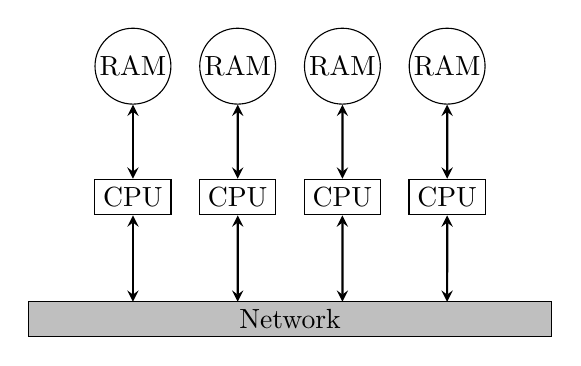
\begin{tikzpicture}[scale=1.33,>=stealth]
      \node[draw, inner sep=3pt] (P0) at (0, 1)  {CPU};
      \node[draw, inner sep=3pt] (P1) at (1, 1)  {CPU};
      \node[draw, inner sep=3pt] (P2) at (2, 1)  {CPU};
      \node[draw, inner sep=3pt] (P3) at (3, 1)  {CPU};

      \node[draw, shape=circle, inner sep=1pt] (R0) at (0, 2.25)  {RAM};
      \node[draw, shape=circle, inner sep=1pt] (R1) at (1, 2.25)  {RAM};
      \node[draw, shape=circle, inner sep=1pt] (R2) at (2, 2.25)  {RAM};
      \node[draw, shape=circle, inner sep=1pt] (R3) at (3, 2.25)  {RAM};

      \filldraw[fill=lightgray] (-1, 0) rectangle node (net) {Network} +(5, -0.33);

      \draw[<->,thick] (P0) edge (0, 0) edge (R0);
      \draw[<->,thick] (P1) edge (1, 0) edge (R1);
      \draw[<->,thick] (P2) edge (2, 0) edge (R2);
      \draw[<->,thick] (P3) edge (3, 0) edge (R3);
    \end{tikzpicture}
  \end{center}

  \begin{itemize}
  \item Each processor has its own memory
    
  \item Communication $=$ messages exchange on a network

  \item Network performance = \textbf{critical} aspect of the machine
  \end{itemize}
\end{frame}

%%%%%%%%%%%%%%%%%%%%%%%%%%%%%%%%%%%%%%%%%%%%%%%%%%%%%%%%%%%%%%%%%%%%

\begin{frame}
  \frametitle{Bad Idea}
  \framesubtitle{Tree-like Ethernet, Ordinary Switches}
  \begin{tikzpicture}
    \path[red, dotted, use as bounding box] (-0.5, 1) rectangle (10, -4.5);
    \node at(5, 0) (switch) {\includegraphics[width=5cm]{old_switch.jpg}};

    \foreach \i in {0, 1, 2, 3, 4, 5} {
      \path (\i*2cm, -3) node {\includegraphics[width=2cm]{gamer.jpg}} edge[->] (switch);
    }
  \end{tikzpicture}

  \bigskip

  Bad performance, scalability problems
  
\end{frame}

\iffalse

%%%%%%%%%%%%%%%%%%%%%%%%%%%%%%%%%%%%%%%%%%%%%%%%%%%%%%%%%%%%%%%%%

\begin{frame}
  \frametitle{Topologie Réseau}
  \framesubtitle{Fat Tree (Infiniband)}

  \centering
  \includegraphics[width=10cm]{fat_tree.pdf}
\end{frame}

%%%%%%%%%%%%%%%%%%%%%%%%%%%%%%%%%%%%%%%%%%%%%%%%%%%%%%%%%%%%%%%

\begin{frame}
  \frametitle{Fat tree (2 levels)}
  
  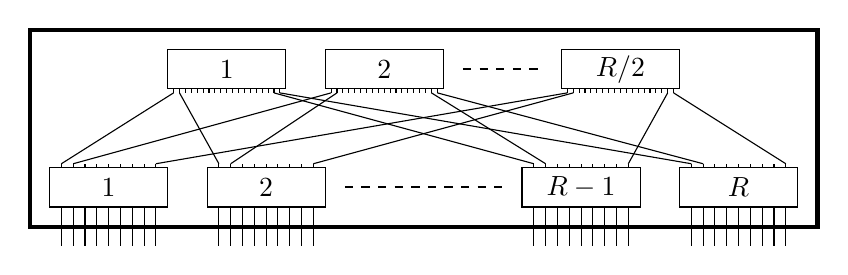
\begin{tikzpicture}[scale=0.5]
  \draw[ultra thick] (-0.5, -0.5) rectangle (19.5, 4.5);
  \draw[dashed, thick] (10.5, 3.5) -- (12.5, 3.5);
  \draw[dashed, thick] (7.5, 0.5) -- (11.5, 0.5);
  
  \foreach \j / \lab in {3/1, 7/2, 13/{$R/2$}} {
    \begin{scope}[xshift=\j*1cm]
      \draw (0, 3) rectangle node {\lab} +(3, 1);
      \foreach \i in {1, 2, ..., 19} {
        \draw (0.15*\i, 3) -- +(0, -0.1);
      }
    \end{scope}
  }

  \foreach \j / \lab in {0/1, 4/2, 12/{$R-1$}, 16/{$R$}} {
    \begin{scope}[xshift=\j*1cm]
      \draw (0, 0) rectangle node {\lab} +(3, 1);
      \foreach \i in {1, 2, ..., 9} {
        \draw (0.3*\i, 0) -- +(0, -1);
        \draw (0.3*\i, 1) -- +(0, 0.1);
      }
    \end{scope}
  }

  \draw (0 + 0.3*1, 1.1) -- (3 + 0.15*1, 2.9);
  \draw (0 + 0.3*2, 1.1) -- (7 + 0.15*1, 2.9);
  \draw (0 + 0.3*9, 1.1) -- (13 + 0.15*1, 2.9);

  \draw (4 + 0.3*1, 1.1) -- (3 + 0.15*2, 2.9);
  \draw (4 + 0.3*2, 1.1) -- (7 + 0.15*2, 2.9);
  \draw (4 + 0.3*9, 1.1) -- (13 + 0.15*2, 2.9);

  \draw (12 + 0.3*1, 1.1) -- (3 + 0.15*18, 2.9);
  \draw (12 + 0.3*2, 1.1) -- (7 + 0.15*18, 2.9);
  \draw (12 + 0.3*9, 1.1) -- (13 + 0.15*18, 2.9);

  \draw (16 + 0.3*1, 1.1) -- (3 + 0.15*19, 2.9);
  \draw (16 + 0.3*2, 1.1) -- (7 + 0.15*19, 2.9);
  \draw (16 + 0.3*9, 1.1) -- (13 + 0.15*19, 2.9);
\end{tikzpicture}

\bigskip

\begin{itemize}
\item Switches \textbf{non-bloquants}
\item Un switch à $R^2 / 2$ ports à partir de $1.5R$ switches à $R$ ports
\item Infiniband : $R = 36 \leadsto $ 648 ports
\end{itemize}

\end{frame}

%%%%%%%%%%%%%%%%%%%%%%%%%%%%%%%%%%%%%%%%%%%%%%%%%%%%%%%%%%%%

\begin{frame}
  \frametitle{Switch infiniband à 648 ports...}
  \centering
  \includegraphics[height=0.75\textheight]{infiniband.png}
\end{frame}

%%%%%%%%%%%%%%%%%%%%%%%%%%%%%%%%%%%%%%%%%%%%%%%%%%%%%%%%%%%%%

\begin{frame}
  \frametitle{Fat tree (3 levels)}
  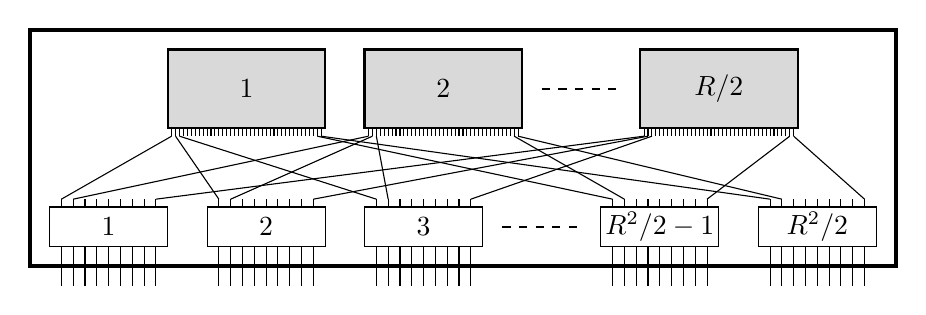
\begin{tikzpicture}[scale=0.5]
   \draw[ultra thick] (-0.5, -0.5) rectangle (21.5, 5.5);
   \draw[dashed, thick] (12.5, 4) -- (14.5, 4);
   \draw[dashed, thick] (11.5, 0.5) -- (13.5, 0.5);
  
  \foreach \j / \lab in {3/1, 8/2, 15/{$R/2$}} {
    \begin{scope}[xshift=\j*1cm]
      \draw[fill=gray!30, thick] (0, 3) rectangle node {\lab} +(4, 2);
      \foreach \i in {1, 2, ..., 39} {
        \draw (0.1*\i, 3) -- +(0, -0.2);
      }
    \end{scope}
  }

  \foreach \j / \lab in {0/1, 4/2, 8/3, 14/{$R^2/2-1$}, 18/{$R^2/2$}} {
    \begin{scope}[xshift=\j*1cm]
      \draw (0, 0) rectangle node {\lab} +(3, 1);
      \foreach \i in {1, 2, ..., 9} {
        \draw (0.3*\i, 0) -- +(0, -1);
        \draw (0.3*\i, 1) -- +(0, 0.2);
      }
    \end{scope}
  }

  \draw (0 + 0.3*1, 1.2) -- (3 + 0.1*1, 2.8);
  \draw (0 + 0.3*2, 1.2) -- (8 + 0.1*1, 2.8);
  \draw (0 + 0.3*9, 1.2) -- (15 + 0.1*1, 2.8);

  \draw (4 + 0.3*1, 1.2) -- (3 + 0.1*2, 2.8);
  \draw (4 + 0.3*2, 1.2) -- (8 + 0.1*2, 2.8);
  \draw (4 + 0.3*9, 1.2) -- (15 + 0.1*2, 2.8);

  \draw (8 + 0.3*1, 1.2) -- (3 + 0.1*3, 2.8);
  \draw (8 + 0.3*2, 1.2) -- (8 + 0.1*3, 2.8);
  \draw (8 + 0.3*9, 1.2) -- (15 + 0.1*3, 2.8);

  
  \draw (14 + 0.3*1, 1.2) -- (3 + 0.1*38, 2.8);
  \draw (14 + 0.3*2, 1.2) -- (8 + 0.1*38, 2.8);
  \draw (14 + 0.3*9, 1.2) -- (15 + 0.1*38, 2.8);

  \draw (18 + 0.3*1, 1.2) -- (3 + 0.1*39, 2.8);
  \draw (18 + 0.3*2, 1.2) -- (8 + 0.1*39, 2.8);
  \draw (18 + 0.3*9, 1.2) -- (15 + 0.1*39, 2.8);
\end{tikzpicture}

\bigskip


\begin{itemize}
\item Même technique en utilisant la construction précédente
\item $R^3 / 4$ ports avec $1.25 R^2$ switches à $R$ ports
\item Infiniband : $R = 36 \leadsto 11 644$ ports
\item Utilisé dans \texttt{Summit} avec 9216 CPUs (un peu de marge)
  \begin{itemize}
  \item 1 baie = 18 noeuds = 36 CPUs = 36 interfaces réseaux
  \item 2 switches 36 ports par baie
  \item 256 baies
  \end{itemize}
\end{itemize}
\end{frame}

%%%%%%%%%%%%%%%%%%%%%%%%%%%%%%%%%%%%%%%%%%%%%%%%%%%%%%%%%%%%%%

\begin{frame}
  \frametitle{Fat tree --- coût élevé du cablage}
  \framesubtitle{Au final, ça ressemble à ça}

  \centering
  \includegraphics[height=8cm]{wiring}

  \bigskip

  Longueur de cable $\geq N^{1.5}$.
\end{frame}


%%%%%%%%%%%%%%%%%%%%%%%%%%%%%%%%%%%%%%%%%%%%%%%%%%%%%%%%%%%%%%%

\begin{frame}
  \frametitle{Topologie Réseau}
  \framesubtitle{Tore 3D (IBM BlueGene/P, Cray XT3, ...)}

  \begin{center}
    \includegraphics[height=6cm]{2x2x2torus.pdf}
  \end{center}

  \begin{itemize}
  \item Longueur de cable proportionnelle à \#CPU
  \item Utilisé sur de très grandes machines (e.g. $48 \times 72 \times 24$)
  \end{itemize}
  
\end{frame}


\begin{frame}
  \frametitle{Topologie Réseau}
  \framesubtitle{Tore 5D (IBM BlueGene/Q)}

  \centering
  \includegraphics[height=8cm]{5D_torus.pdf}
\end{frame}

\begin{frame}
  \frametitle{Topologie Réseau}
  \framesubtitle{Dragonfly (Cray ``Aries'' interconnect)}

  \centering
  \includegraphics[height=8cm]{dragonfly.pdf}
\end{frame}
\fi


%%%%%%%%%%%%%%%%%%%%%%%%%%%%%%%%%%%%%%%%%%%%%%%%%%%%%%%%%%%%%%%%%%%%%

\begin{frame}
  \frametitle{Shared Memory}

  \begin{center}
    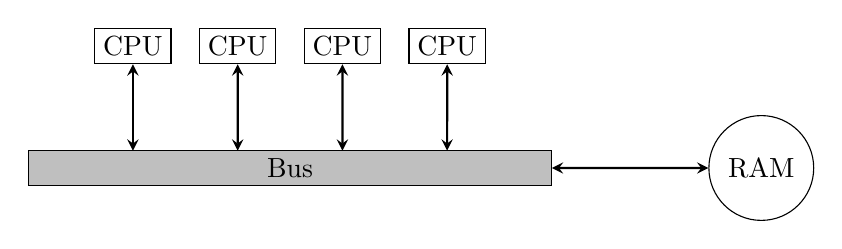
\begin{tikzpicture}[scale=1.33,>=stealth]
      \node[draw, inner sep=3pt] (P0) at (0, 1)  {CPU};
      \node[draw, inner sep=3pt] (P1) at (1, 1)  {CPU};
      \node[draw, inner sep=3pt] (P2) at (2, 1)  {CPU};
      \node[draw, inner sep=3pt] (P3) at (3, 1)  {CPU};

      \node[draw, shape=circle, inner sep=5pt] (R0) at (6, -0.33/2)  {RAM};

      \filldraw[fill=lightgray] (-1, 0) rectangle node (net) {Bus} +(5, -0.33);

      \draw[<->,thick] (P0) edge (0, 0);
      \draw[<->,thick] (P1) edge (1, 0);
      \draw[<->,thick] (P2) edge (2, 0);
      \draw[<->,thick] (P3) edge (3, 0);
      
      \draw[<->,thick] (R0) edge (4, -0.33 / 2);
    \end{tikzpicture}
  \end{center}

  
  \begin{itemize}
    
  \item CPUs connected to the memory through a bus
    
  \item Each CPU may access the whole memory
    
  \item Communications $\leftrightarrow $ memory accesses    
  \end{itemize}

  \bigskip
  \begin{itemize}
  \item Beware of race conditions!
  \end{itemize}  
\end{frame}

% %%%%%%%%%%%%%%%%%%%%%%%%%%%%%%%%%%%%%%%%%%%%%%%%%%%%%%%%%%%%%%%%%%%%%
% \begin{frame}
%   \frametitle{Mémoire partagée}
%   \framesubtitle{Classification selon l'organisation de la mémoire}


%   \begin{block}{{\it Race condition :}}
%     Il y a {\it race condition} lorsque  
%     \begin{itemize}
%     \item au moins 2 processeurs accèdent à la même variable
%     \item au moins un processeur y accède en écriture 
%     \item ces accès sont potentiellement concurrents (ils peuvent
%       être effectués ``au même moment'')
%     \end{itemize}
%   \end{block}
  
%   \medskip
  
%   \mintinline{C}{i = i + 1;}
  
%   \medskip
  
%   \begin{exampleblock}{Solution}
%     mécanismes de synchronisation (section critique,
%     opération atomique, barrière de synchronisation)
%   \end{exampleblock}
% \end{frame}


%%%%%%%%%%%%%%%%%%%%%%%%%%%%%%%%%%%%%%%%%%%%%%%%%%%%%%%%%%%%%%%%%

\begin{frame}
  \frametitle{Non-Uniform Memory Access}

  \begin{alertblock}{Shared memory: scalability problem}
    More CPUS $\leadsto$ contention on the bus
  \end{alertblock}

  \begin{exampleblock}{Solution}
    \begin{itemize}
    \item Simulate a shared memory with a distributed memory
    \item Each CPU ``owns'' and control a share of the memory
      \begin{itemize}
      \item \emph{Directly} accesses its own share 
      \end{itemize}
    \item Accesses the rest by communicating with other CPUs
    \item[$\Rightarrow$] \textit{ad hoc} network, very fast.
    \end{itemize}
  \end{exampleblock}
\end{frame}

%%%%%%%%%%%%%%%%%%%%%%%%%%%%%%%%%%%%%%%%%%%%%%%%%%%

\begin{frame}
  \frametitle{Non-Uniform Memory Access}
  \framesubtitle{Real Example}

  \begin{itemize}
  \item SMP node with $2 \times$ AMD EYPC ``Naples'' CPUs
  \item 4 $\times$ independent memory controller per CPU
  \item<3-> Complete interconnection inside of a CPU
  \item<4-> Partial interconnection between the two sockets
  \item<4-> Red link = $\approx 2\times$ higher latency
  \end{itemize}

  \medskip

    \begin{center}
      \begin{tikzpicture}[scale=1.33,>=stealth]
        \path[use as bounding box] (-3, -2.25) rectangle +(6, 4);
        \node at (0, -0.15) {\includegraphics[width=\textwidth]{lstopo_chiclet}};
        
        \node<2->[draw, ultra thick, fill=white, inner sep=5pt] (P2) at (-3, -1)  {$P_2$};
        \node<2->[draw, ultra thick, fill=white, inner sep=5pt] (P0) at (-3, 0.5)  {$P_0$};
        \node<2->[draw, ultra thick, fill=white, inner sep=5pt] (P3) at (-1, -1)  {$P_3$};
        \node<2->[draw, ultra thick, fill=white, inner sep=5pt] (P1) at (-1, 0.5)  {$P_1$};
        \node<2->[draw, ultra thick, fill=white, inner sep=5pt] (P6) at (1, -1)  {$P_6$};
        \node<2->[draw, ultra thick, fill=white, inner sep=5pt] (P4) at (1, 0.5)  {$P_4$};
        \node<2->[draw, ultra thick, fill=white, inner sep=5pt] (P7) at (3, -1)  {$P_7$};
        \node<2->[draw, ultra thick, fill=white, inner sep=5pt] (P5) at (3, 0.5)  {$P_5$};

        \node<2->[draw, shape=circle,ultra thick, fill=white, inner sep=1pt] (M2) at (-3.25, -2)  {$M_2$};
        \node<2->[draw, shape=circle,ultra thick, fill=white, inner sep=1pt] (M0) at (-3.25, 1.5)  {$M_0$};
        \node<2->[draw, shape=circle,ultra thick, fill=white, inner sep=1pt] (M3) at (-1.25, -2)  {$M_3$};
        \node<2->[draw, shape=circle,ultra thick, fill=white, inner sep=1pt] (M1) at (-1.25, 1.5)  {$M_1$};
        \node<2->[draw, shape=circle,ultra thick, fill=white, inner sep=1pt] (M6) at (1.25, -2)  {$M_6$};
        \node<2->[draw, shape=circle,ultra thick, fill=white, inner sep=1pt] (M4) at (1.25, 1.5)  {$M_4$};
        \node<2->[draw, shape=circle,ultra thick, fill=white, inner sep=1pt] (M7) at (3.25, -2)  {$M_7$};
        \node<2->[draw, shape=circle,ultra thick, fill=white, inner sep=1pt] (M5) at (3.25, 1.5)  {$M_5$};

        \draw<3->[ultra thick,<->] (P0) edge (P1) edge (P2) edge (P3);
        \draw<3->[ultra thick,<->] (P1) edge (P2) edge (P3);
        \draw<3->[ultra thick,<->] (P2) edge (P3);
        \draw<3->[ultra thick,<->] (P4) edge (P5) edge (P6) edge (P7);
        \draw<3->[ultra thick,<->] (P5) edge (P6) edge (P7);
        \draw<3->[ultra thick,<->] (P6) edge (P7);
        \draw<4>[ultra thick,red,<->] (P2) edge[bend right=2cm] (P4);
        \draw<4>[ultra thick,red,<->] (P3) edge[bend left=2cm] (P5);
        \draw<4>[ultra thick,red,<->] (P0) edge[bend right=2cm] (P6);
        \draw<4>[ultra thick,red,<->] (P1) edge[bend left=2cm] (P7);

        \draw<2->[ultra thick,dotted] (P0) edge (M0);
        \draw<2->[ultra thick,dotted] (P1) edge (M1);
        \draw<2->[ultra thick,dotted] (P2) edge (M2);
        \draw<2->[ultra thick,dotted] (P3) edge (M3);
        \draw<2->[ultra thick,dotted] (P4) edge (M4);
        \draw<2->[ultra thick,dotted] (P5) edge (M5);
        \draw<2->[ultra thick,dotted] (P6) edge (M6);
        \draw<2->[ultra thick,dotted] (P7) edge (M7);
        
      \end{tikzpicture}
  \end{center}
\end{frame}

%%%%%%%%%%%%%%%%%%%%%%%%%%%%%%%%%%%%%%%%%%%%%%%%%%%

\begin{frame}
  \frametitle{In practice...}

  \begin{itemize}
  \item machine = nodes connected to a network
    \begin{itemize}
      \item MIMD / distributed memory
    \end{itemize}
    \medskip
  \item One node = several processors (SMP)
    \begin{itemize}
    \item Most likely NUMA
    \end{itemize}
    \medskip
  \item Inside a node = all cores access the memory
    \begin{itemize}
    \item Shared memory
    \end{itemize}
    \medskip
  \item Inside a core = vector instructions
    \begin{itemize}
    \item SIMD
    \end{itemize}
  \end{itemize}

  \bigskip

  Everything, everywhere, all the time.
\end{frame}

%%%%%%%%%%%%%%%%%%%%%%%%%%%%%%%%%%%%%%%%%%%%%%%%%%%%%%%%

\begin{frame}[fragile]
  \frametitle{Instruction-Level Parallelism (ILP)}

  \begin{columns}
    \begin{column}{3cm}  
\begin{minted}{gas}
slwi 10,9,3
add 8,11,10
lwzx 10,11,10
lwz 7,4(8)
or. 10,10,7
bne 0,.L146
addi 5,5,8
stw 3,0(8)
stw 4,4(8)
cmplw 7,6,5
bne 7,.L24
lwz 9,144(19)
li 10,1
stw 10,20704(31)
addi 9,9,1
\end{minted}
%stw 9,144(19)
    \end{column}  

    \begin{column}{7cm}
      code = \emph{ordered} sequence of instructions

      \medskip

      \begin{alertblock}{Parallelism inside a core}
      \begin{itemize}
      \item \emph{Pipeline(s)}
      \item \emph{Superscalarity}
      \item \emph{Out-of-order execution}
      \item \emph{Simultaneous Multi-Threading}
      \end{itemize}
    \end{alertblock}

    \begin{itemize}
    \item[$\Rightarrow$] Parallel implementation
    \item[$\Rightarrow$] Sequential semantics
    \end{itemize}
    
    \end{column}
  \end{columns}
\end{frame}

%%%%%%%%%%%%%%%%%%%%%%%%%%%%%%%%%%%%%%%%%%%%%%%%%%%%%%%%%%%%%%%%%%%%%

\begin{frame}[fragile]
  \frametitle{How to Write Parallel Programs?}

  \begin{itemize}
  \item<1-> Automatic parallelization
  \item<2-> ``Annotations'' and compiler hints in C programs  (\red{OpenMP}, OpenACC)
  \item<3-> plain C + libraries (\texttt{pthread}, \red{MPI})
  \item<4-> New languages?
  \end{itemize}

  \medskip

  \begin{overlayarea}{\textwidth}{5cm}
  \begin{block}<only@2>{OpenMP}
\begin{minted}{C}
#pragma omp parallel for
for (int i = 0; i < n; i++)
    for (int j = 0; j < n; j++)
        for (int k = 0; k < n; k++)
            C[i][j] += A[i][k] * B[k][j];
\end{minted}
  \end{block}


  \begin{block}<only@3>{Librairies}
\begin{minted}[fontsize=\scriptsize]{C}
 for(int t=0; t<NUM_THREADS; t++)
       pthread_create(&threads[t], NULL, ThreadFunction, (void *) t);
...
pthread_exit();
\end{minted}
  \end{block}

  \begin{block}<only@4>{Go}
\begin{minted}[fontsize=\small]{go}
func main() {
    s := []int{7, 2, 8, -9, 4, 0}
    c := make(chan int)
    go sum(s[:len(s)/2], c)
    go sum(s[len(s)/2:], c)
    x, y := <-c, <-c
    fmt.Println(x, y, x+y)
}
\end{minted}
  \end{block}
\end{overlayarea}
\end{frame}


%%%%%%%%%%%%%%%%%%%%%%%%%%%%%%%%%%%%%%%%%%%%%%%%%%%%%%%%%%%%%%%%%%%%% 


\begin{frame}[fragile]
  \frametitle{Recycling Sequential Programming Languages}


  \begin{block}{\emph{Single Program Multiple Data} (SPMD)}
    \begin{itemize}
    \item Same sequential code executed many times in parallel
    \item Special variable: \texttt{rank}
    \item $\texttt{rank} = i$ in the $i$-th copy of the program
    \end{itemize}
  \end{block}

  \medskip
  
  \begin{minted}{C}
int i = rank;                /* data parallelism */
for (int j = 0; j < n; j++)
    for (int k = 0; k < n; k++)
        C[i][j] += A[i][k] * B[k][j];

if (rank == 0) {             /* control parallelism */
  <<Purely sequential section>>
} else {
  <<Wait>>
}
\end{minted}
\end{frame}

%%%%%%%%%%%%%%%%%%%%%%%%%%%%%%%%%%%%%%%%%%%%%%%%%%%%%%%%%%%%%%%%%%%%

\begin{frame}
\frametitle{Performance Evaluation}

Justice of the peace : \alert{wall clock}

\medskip

\begin{itemize}
\item $T_1(n)$: time needed by the \textbf{best} sequential algorithm
  to process an instance of size $n$

  \medskip
  
\item $T_p(n)$: time needed by the parallel algorithm   to process an instance of size $n$ on $p$ processors
\end{itemize}

\vspace*{-0.5cm}
\begin{columns}[t]

\column{0.5\textwidth}
\begin{block}{\textbf{Speedup}}
  \[
    S(n,p)  =  \frac{T_1(n)}{T_p(n)}
  \]
\end{block}

\column{0.5\textwidth}
\begin{block}{\textbf{Efficiency}}
  \[
    E(n,p)  = \frac{S(n,p)}{p}
  \]
\end{block}
\end{columns}
\end{frame}


%%%%%%%%%%%%%%%%%%%%%%%%%%%%%%%%%%%%%%%%%%%%%%%%%%%%%%%%%%%%%%%%%%%%%
\begin{frame}
\frametitle{Strong scaling}

\begin{alertblock}{Goal when Parallelizing?}
  \begin{itemize}
  \item \textbf{Minimize time-to-solution for a fixed problem}
  \item[$\Rightarrow$] Study of the performance with fixed $n$ and increasing $p$
  \end{itemize}
\end{alertblock}

\medskip

\begin{itemize} 
\item  \textbf{Linear speedup ($\rightarrow$ ideal):} 
processors are 100\% busy, no extra operations
\[
  S(n,p)  = p \qquad E(n,p)  = 1
\]

\medskip

\item \textbf{Sublinear speedup:}
processors are less than~100\% busy, or extra operations 

\medskip

\item {\bf Superinear speedup:} hard to envision 


\end{itemize}
\end{frame}




%%%%%%%%%%%%%%%%%%%%%%%%%%%%%%%%%%%%%%%%%%%%%%%%%%%%%%%%%%%%%%%%%%%%%
\begin{frame}
  \frametitle{Strong scaling}
  \framesubtitle{Real example}
  
  \begin{columns}
    \begin{column}{0.4\textwidth}
      \begin{center}
        \begin{tikzpicture}
          \path[use as bounding box] (-0.2, -0.5) rectangle +(4.2, 4.8);
          \draw[thick,->] (-0.15, 0.075) -- node[above,sloped] {Time} +(0, 4.7);
          \draw[thick,->] (0, -0.15) -- node[below] {Processors} +(4.3, 0);
          \node[anchor=south west,inner sep=0] at (0, 0) {\includegraphics[width=\textwidth]{strong.png}};
        \end{tikzpicture}
        
        {\tiny (M.J. Quinn)}
      \end{center}
    \end{column}
    
    \begin{column}{0.63\textwidth}
      \begin{itemize}
      \item Gray: computation time
        \begin{itemize}
        \item decreases (or stagnate) when $p \nearrow$
        \end{itemize}

        \medskip
        
      \item White: overhead
        \begin{itemize}
        \item Increases when $p \nearrow$
        \end{itemize}

        \medskip
        
      \item For a given problem size ($n$), there is an optimal number of processors that can be efficiently exploited
        \begin{itemize}
        \item Beyond this point, adding extra processors no longer bring any gain
        \end{itemize}
      \end{itemize}
    \end{column}
  \end{columns}  
\end{frame}

%%%%%%%%%%%%%%%%%%%%%%%%%%%%%%%%%%%%%%%%%%%%%%%%%%%%%%%%%%%%%%%%%%%%%

\begin{frame}
\frametitle{Real Example (my code)}
\framesubtitle{Compute Rank of Sparse Integer Matrices}

\centering
\includegraphics[height=6cm]{d19.pdf}

\medskip

\small
  \begin{tabular}{|c|c|l|c|c|}
\hline
Name & CPU Type        & \# CPU     & cores/CPU & L3 Cache/CPU\\
\hline\hline
A    & Xeon E5-2670 v3 & $2 \times$ & 12        & 30MB\\
\hline
B    & Xeon E5-4620    & $4 \times$ & 8         & 16MB\\
\hline
C    & Xeon E5-2695 v4 & $2 \times$ & 18        & 45MB\\
\hline
\end{tabular}



\end{frame}

%%%%%%%%%%%%%%%%%%%%%%%%%%%%%%%%%%%%%%%%%%%%%%%%%%%%%%%%%%%%%%%%%%%%%

\begin{frame}
  \frametitle{Amdahl's Law}
  \framesubtitle{Sequential Portions Limit Parallel Speedup}

  An Algorithm with a fraction $f$ of operations that must be performed
  sequentially. Then

\[
  S(n,p)  \leq  \frac{1}{f + (1 - f)/p}
\]

$\Rightarrow$ 20\% of an algorithm is sequential $\leadsto$ Speedup $\leq 5$

\bigskip

Overhead caused by parallelism ($1 - E(n,p)$) 
caused by sequential parts and
\begin{itemize}
\item Communications
\item Starting / Synchronizing tasks 
\item Load imbalance
\item ...
\end{itemize}

\end{frame}

%%%%%%%%%%%%%%%%%%%%%%%%%%%%%%%%%%%%%%%%%%%%%%%%%%%%%%%%%%%%%%%%%%%%%
\begin{frame}
\frametitle{Weak scaling}

\begin{alertblock}{Goal when Parallelizing?}
  \begin{itemize}
  \item \textbf{Solve \emph{bigger} problems with more processors}
  \item[$\Rightarrow$] Study of the performance when both $p$ and $n$ increase
  \end{itemize}
\end{alertblock}

\medskip

\begin{exampleblock}{Amdahl's effect (empirical)}
\begin{itemize}
\item When $n \nearrow$, computation time often increase \emph{more} that communication time
\item Often allows for greater speedups
\end{itemize}
\end{exampleblock}
\end{frame}

%%%%%%%%%%%%%%%%%%%%%%%%%%%%%%%%%%%%%%%%%%%%%%%%%%%%%%%%%%%

\begin{frame}
  \frametitle{Gustafson-Barsis's Law}

  On exécute un programme parallèle sur $p$ processeurs.

  \medskip
  
  A parallel computation is run ; time spent in sequential operations is measured and represents a fraction $s$ of the total.

  \medskip
  
  Alors :
  \[
    S(n, p) \leq  p - (p-1)s
  \]

    \medskip
  
    \begin{block}{Example}
      A parallel computation runs in 100s on 32 processors, including 5s in serial portions.
      Then $S(n, p) \leq 30.45$.
    \end{block}
  \end{frame}


%%%%%%%%%%%%%%%%%%%%%%%%%%%%%%%%%%%%%%%%%%%%%%%%%%%%%%%%%%%%%%%

\end{document}

% Charles' emacs magic commands
%%% Local Variables:
%%% TeX-engine: xetex
%%% TeX-command-extra: "-shell-escape"
%%% TeX-command-extra-options: "-shell-escape"
%%% ispell-local-dictionary: "english"
%%% eval: (flyspell-mode 1)
%%% eval: (reftex-mode 1)
%%% End:
